% Created 2015-03-12 Thu 18:23
\documentclass[11pt]{article}
\usepackage[latin1]{inputenc}
\usepackage[T1]{fontenc}
\usepackage{fixltx2e}
\usepackage{graphicx}
\usepackage{longtable}
\usepackage{float}
\usepackage{wrapfig}
\usepackage{rotating}
\usepackage[normalem]{ulem}
\usepackage{amsmath}
\usepackage{textcomp}
\usepackage{marvosym}
\usepackage{wasysym}
\usepackage{amssymb}
\usepackage{hyperref}
\tolerance=1000
\usepackage[parfill]{parskip}
\usepackage{mathtools}
\usepackage[utf8]{inputenc}
\usepackage[swedish, english]{babel}
\usepackage[T1]{fontenc}
\usepackage{moreverb,fancyheadings,graphicx, amssymb}
\usepackage{fixltx2e}
\usepackage{longtable}
\usepackage{float}
\usepackage{wrapfig}
\usepackage{soul}
\usepackage{textcomp}
\usepackage{marvosym}
\usepackage{wasysym}
\usepackage{latexsym}
\usepackage{hyperref}
\author{Anton Erholt \& Christopher M�rtensson \\ <aerholt@kth.se> <cmarte@kth.se>}
\date{\today}
\title{Parallelized particle simulation}
\hypersetup{
  pdfkeywords={},
  pdfsubject={A project in the course ID1217 at KTH},
  pdfcreator={Emacs 24.4.1 (Org mode 8.2.10)}}
\begin{document}

\maketitle
\newpage
\begin{abstract}

This report serves to describe a programming project in the course
ID1217, Concurrent programming. The project was to implement an
algorithm for a parallel particle simulation which ran in time close to $O(T/p)$,
where $T$ is the running time of the algorithm running on $p$ processors.

\end{abstract}
\newpage

\section*{Introduction}
\label{sec-1}

This programming project is about finding an improved algorithm for
solving a particle simulation problem and implementing
it. Furthermore, the project consists of improving said implementation
by parallelizing it to several processors.

The particle simulation is made by a per-particle basis, applying the
force of its neighboring particles and recalculating the particle
position and velocity.

\section*{The algorithm}
\label{sec-2}

The algorithm we have chosen to implement is probably best known as
binning. We divide the field of particles into several 'bins' (like a
grid) which we then use to filter out which particles we need to take
into account when calculating forces. Using a shared memory layout
with this type of design requires little to no changes for an actual
implementation. With a distributed memory layout, the design requires
a few additions.

The algorithm described in pseudo-code is:

\begin{verbatim}
P = set(Particle)
N = P.size()

def simulate_step():
    for particle in P:
        # Parallelize here
        neighbors = find_neighbors(particle)
        for n in neighbors:
            particle.applyForceOf(n)
    # Synchronize here
    for particle in P:
        particle.move()
    # Synchronize here
\end{verbatim}

Where the size of neighbors is significantly smaller than N and
therefore makes the binning algorithm's running time $\in O(N)$.

$$ neighbors.size() << N $$

The calculation part which we parallelize is obviously the force calculation and the move calculation for
every particle. This project limits itself not to discuss whether or
not one would gain anything from also parallelizing over time
steps.

\section*{Implementation details}
\label{sec-3}

\subsection*{Shared memory layout}
\label{sec-3-1}

\subsubsection*{Serial}
\label{sec-3-1-1}
The serial solution uses no type of parallelization and runs the
binning algorithm as described above, in $O(n)$ time (where $n$ is the number
of particles).

\subsubsection*{OpenMP}
\label{sec-3-1-2}
The OpenMP version implements a parallel version of the binning
algorithm. It uses the \verb~#pragma omp parallel for~ directive for
parallelization and synchronization. The directive \verb~#pragma omp critical~ is used to ensure the critical regions of the algorithm is
executed atomically.

\subsubsection*{Pthreads}
\label{sec-3-1-3}
The pthreads implementation uses lower level synchronization
primitives, namely a barrier for synchronization and a mutex for
locking. The particle array is split into as many chunks as we have
threads, and each thread gets to work on its own chunk.

\subsection*{Distributed memory layout}
\label{sec-3-2}

Using a distributed memory layout forces an addition in the algorithm
design. Instead of each process being responsible for a certain set of
particles as in the shared memory model, each process is instead
responsible for a 'region' in space, or equivalently a certain set of
'bins'. First, we distribute the 'bins' over the different processes.
In our case, this is done vertically, so a process is in charge of all
particles in a certain range in y-coordinates. During the force
calculation, each process sends information about the particles in the
topmost and bottommost bins to its neighboring processes for them to
be able to perform the force calculation. After the move calculation
has been performed, the particles that moved into another processes'
region is sent to that process. This algorithm is expressed in the
following pseudocode:

\begin{verbatim}
R = get_region()
P = particles_in(R)
N = P.size()

def simulate_step():
    # Get neighboring particles from other processes here
    # Apply force
    for particle in P:
        neighbors = find_neighbors(particle)
        for n in neighbors:
            particle.applyForceOf(n)
    # Move particles
    for particle in P:
        particle.move()
    # Send particles that moved into other regions to the owning process of that region here
\end{verbatim}

The message passing is done synchronously, due to risk of buffer
overflow when using asynchronous. In order to prevent deadlocking, the
message-passing is done in order; on the first pass messages are sent
from the first process to the last, and then back again from the last
to the first.



\subsubsection*{MPI}
\label{sec-3-2-1}
We estimate the contention of our implementation to be quite high, but
still being able to beat the non-linear implementation given.

\section*{Measurements, calculations and plots}
\label{sec-4}

\subsection*{Linearity}
\label{sec-4-1}
By plotting the size of the input $n$ and the running time
$t_serial$ we conclude the linearity of our algorithm.

See Appendix for output of the actual runs.

\begin{center}
\begin{tabular}{rrrr}
n & t$_{\text{serial}}$ & log$_{\text{2}}$(t$_{\text{serial}}$) & log$_{\text{2}}$(n)\\
\hline
5000 & 2.530250 & 0.84499156 & 12.28771238\\
10000 & 5.798080 & 1.599769861 & 13.28771238\\
20000 & 9.404700 & 2.040036861 & 14.28771238\\
40000 & 23.231000 & 2.863146195 & 15.28771238\\
80000 & 54.164900 & 3.633705119 & 16.28771238\\
160000 & 110.290000 & 4.280958177 & 17.28771238\\
\end{tabular}
\end{center}

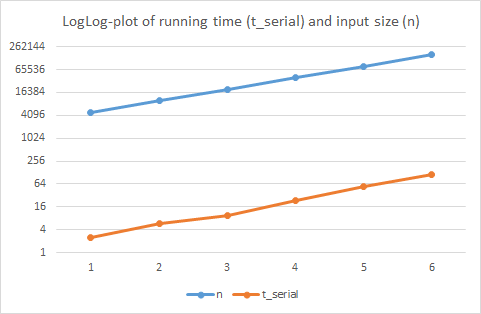
\includegraphics[width=.9\linewidth]{./loglog-serial.png}

\newpage
\subsection*{Comparison of running times}
\label{sec-4-2}

\subsection*{Serial, running on u-shell.csc.kth.se}
\label{sec-4-3}

\begin{verbatim}
particles = 4000, simulation time = 0.459393 seconds
particles = 8000, simulation time = 0.9433 seconds
particles = 16000, simulation time = 3.00457 seconds
particles = 32000, simulation time = 8.81252 seconds
particles = 64000, simulation time = 19.3659 seconds
particles = 40000, simulation time = 11.2636 seconds
\end{verbatim}

\subsection*{Pthreads, running on u-shell.csc.kth.se}
\label{sec-4-4}

\begin{verbatim}
processes = 2, particles = 40000, simulation time = 22.8733 seconds
processes = 4, particles = 40000, simulation time = 12.5229 seconds
processes = 8, particles = 40000, simulation time = 8.96185 seconds
\end{verbatim}

\subsection*{OpenMP, running on u-shell.csc.kth.se}
\label{sec-4-5}

\begin{verbatim}
processes = 2, particles = 40000, simulation time = 6.35436 seconds
processes = 4, particles = 40000, simulation time = 3.55033 seconds
processes = 8, particles = 40000, simulation time = 3.12963 seconds
\end{verbatim}

\subsection*{MPI, running on u-shell.csc.kth.se}
\label{sec-4-6}

\begin{verbatim}
processes = 2, particles = 40000, simulation time = 9.17019 seconds
processes = 4, particles = 40000, simulation time = 6.37624 seconds
processes = 8, particles = 40000, simulation time = 6.16595 seconds
\end{verbatim}

\section*{Discussion and thoughts}
\label{sec-5}

\subsection*{PTHREADS}
\label{sec-5-1}
The implementation using pthreads was pretty straight forward. We
expected it to perform way better and believe it to be the
synchronization stealing a lot of the CPU-time. An extension of this
project would go into detail of investigating this issue further.

\subsection*{OPENMP}
\label{sec-5-2}
In terms of ease of use, openMP was by far the best of the methods. It
literally took no more than 4 extra lines of code in the serial
version of the program to parallelize it. From the results we also see
that this method was the most effective, and the only one that
actually performed better than the serial implementation.

\subsection*{MPI}
\label{sec-5-3}
The amount of contention in the MPI implementation was quite large
since information about neighboring particles was needed to be
constantly be sent at each iteration. This meant that the time needed
to perform the particle physics computations was quite small compared
to the amount of time spent on message passing. A distributed memory
model was perhaps not the most well suited model for this problem,
since the memory required (the particle data) was not independent
between processes but rather, in order for a process to be able to
process its own particles it required information about another
process' particles. Thus, if one is concerned more about memory usage
than about speed, this model would be more effective, but in our case
it quickly reached a bottleneck in speed for higher number of
processes.
\newpage
\section*{Appendix}
\label{sec-6}

\subsection*{Output of running linearserial (for 'proving' linearity)}
\label{sec-6-1}

\textbf{NOTE:} Some runs are omitted below. This is just an excerpt from were
the calculation numbers were taken.

\begin{verbatim}
[aerholt@localhost particles-pps14]$ ./linearserial -n 5000
size: 7.071068
integer size: 317
Scale: 44.830570
n = 5000, simulation time = 1.94145 seconds
[aerholt@localhost particles-pps14]$ ./linearserial -n 5000
size: 7.071068
integer size: 317
Scale: 44.830570
n = 5000, simulation time = 2.10103 seconds
[aerholt@localhost particles-pps14]$ ./linearserial -n 5000
size: 7.071068
integer size: 317
Scale: 44.830570
n = 5000, simulation time = 2.53025 seconds
[aerholt@localhost particles-pps14]$ ./linearserial -n 5000
size: 7.071068
integer size: 317
Scale: 44.830570
n = 5000, simulation time = 2.58599 seconds
[aerholt@localhost particles-pps14]$ ./linearserial -n 5000
size: 7.071068
integer size: 317
Scale: 44.830570
n = 5000, simulation time = 2.54449 seconds
[aerholt@localhost particles-pps14]$ ./linearserial -n 10000
size: 10.000000
integer size: 448
Scale: 44.800000
n = 10000, simulation time = 5.79808 seconds
[aerholt@localhost particles-pps14]$ ./linearserial -n 10000
size: 10.000000
integer size: 448
Scale: 44.800000
n = 10000, simulation time = 5.81343 seconds
[aerholt@localhost particles-pps14]$ ./linearserial -n 10000
size: 10.000000
integer size: 448
Scale: 44.800000
n = 10000, simulation time = 5.73867 seconds
[aerholt@localhost particles-pps14]$ ./linearserial -n 10000
size: 10.000000
integer size: 448
Scale: 44.800000
n = 10000, simulation time = 5.61922 seconds
[aerholt@localhost particles-pps14]$ ./linearserial -n 10000
size: 10.000000
integer size: 448
Scale: 44.800000
n = 10000, simulation time = 6.2238 seconds
[aerholt@localhost particles-pps14]$ ./linearserial -n 20000
size: 14.142136
integer size: 633
Scale: 44.759859
n = 20000, simulation time = 9.4047 seconds
[aerholt@localhost particles-pps14]$ ./linearserial -n 20000
size: 14.142136
integer size: 633
Scale: 44.759859
n = 20000, simulation time = 8.65654 seconds
[aerholt@localhost particles-pps14]$ ./linearserial -n 40000
size: 20.000000
integer size: 895
Scale: 44.750000
n = 40000, simulation time = 31.0985 seconds
[aerholt@localhost particles-pps14]$ ./linearserial -n 40000
size: 20.000000
integer size: 895
Scale: 44.750000
n = 40000, simulation time = 23.231 seconds
[aerholt@localhost particles-pps14]$ ./linearserial -n 40000
size: 20.000000
integer size: 895
Scale: 44.750000
n = 40000, simulation time = 25.2277 seconds
[aerholt@localhost particles-pps14]$ ./linearserial -n 80000
size: 28.284271
integer size: 1265
Scale: 44.724504
n = 80000, simulation time = 60.2246 seconds
[aerholt@localhost particles-pps14]$ ./linearserial -n 80000
size: 28.284271
integer size: 1265
Scale: 44.724504
n = 80000, simulation time = 49.7609 seconds
[aerholt@localhost particles-pps14]$ ./linearserial -n 80000
size: 28.284271
integer size: 1265
Scale: 44.724504
n = 80000, simulation time = 54.1649 seconds
[aerholt@localhost particles-pps14]$ ./linearserial -n 160000
size: 40.000000
integer size: 1789
Scale: 44.725000
n = 160000, simulation time = 115.779 seconds
[aerholt@localhost particles-pps14]$ ./linearserial -n 160000
size: 40.000000
integer size: 1789
Scale: 44.725000
n = 160000, simulation time = 110.29 seconds
\end{verbatim}

\subsection*{Profiling of linpthreads}
\label{sec-6-2}

Please see "pthreads-profile" in kcachegrind or similar.
% Emacs 24.4.1 (Org mode 8.2.10)
\end{document}
